% Biology

\chapter{Local Materials List}
\label{cha:local-materials}

In order to gain a thorough understanding of science, students must be able to make a connection between classroom learning and the outside world. The following is a list of locally available materials which may be used to substitute conventional materials and apparatus for various activities. These materials have the following advantages: 
\begin{itemize*}
\item They are readily available in the village or a nearby town;
\item They are cheaper than conventional materials; 
\item They may safely substitute the conventional materials without fear of losing accuracy or understanding; 
\item They help students to draw a connection between science education and the world around them.
\end{itemize*}
Imagination and innovativeness is encouraged on the part of the student and teacher to find other suitable local substitutions. 

Below are common apparatus you might order from a laboratory supply company, 
and comments about which have good if not superior alternatives 
available in villages and towns. 
Given equal quality, 
it is generally better to use local materials, 
because these help connect classroom learning to students' lives.\\

The apparatus listed in this section are the following:

\begin{multicols}{3}

\begin{enumerate}
%\item \nameref{sec:alligator-clips}
\item \nameref{sec:balance}
\item \nameref{sec:beakers}
\item \nameref{sec:blowpipe}
%\item \nameref{sec:lightbulbs}
\item \nameref{sec:bunsen-burner}
\item \nameref{sec:burettes}
%\item \nameref{sec:circuit-comp}
\item \nameref{sec:crucible}
%\item \nameref{sec:condenser}
\item \nameref{sec:containers}
\item \nameref{sec:deflagratingspoon}
\item \nameref{sec:delivery-tube}
\item \nameref{sec:drawing-board}
\item \nameref{sec:droppers}
\item \nameref{sec:electrodes}
%\item \nameref{sec:electrode-holder}
%\item \nameref{sec:electrolytic-cell}
%\item \nameref{sec:eureka-can}
\item \nameref{sec:filter-paper}
\item \nameref{sec:flasks}
\item \nameref{sec:funnel}
%\item \nameref{sec:glass-blocks}
\item \nameref{sec:gloves}
\item \nameref{sec:goggles}
\item \nameref{sec:heatsources}
\item \nameref{sec:indicator}
\item \nameref{sec:iron-filings}
\item \nameref{sec:masses}
\item \nameref{sec:meascyl}
\item \nameref{sec:meter-rule}
\item \nameref{sec:microscope}
%\item \nameref{sec:mirrors}
\item \nameref{sec:mortar-and-pestle}
%\item \nameref{sec:nichrome-wire}
\item \nameref{sec:optical-pins}
\item \nameref{sec:pipettes}
%\item \nameref{sec:pulleys}
%\item \nameref{sec:resistors}
\item \nameref{sec:retort-stand}
\item \nameref{sec:scale-pan}
\item \nameref{sec:scalpels}
\item \nameref{sec:slide-cover-slip}
\item \nameref{sec:spatula}
%\item \nameref{sec:spring-balance}
%\item \nameref{sec:springs}
\item \nameref{sec:stoppers}
\item \nameref{sec:stopwatches}
\item \nameref{sec:testtubes}
\item \nameref{sec:test-tube-brush}
\item \nameref{sec:test-tube-holder}
\item \nameref{sec:test-tube-racks}
\item \nameref{sec:tripod-stands}
\item \nameref{sec:volumetric-glassware}
\item \nameref{sec:wash-bottle}
\item \nameref{sec:hotwaterbathes}
\item \nameref{sec:weights}
\item \nameref{sec:white-tiles}
%\item \nameref{sec:wire}
\item \nameref{sec:wire-gauze}
\end{enumerate}

\end{multicols}

\pagebreak

How many experiments can be carried out with everyday items?

\begin{center}
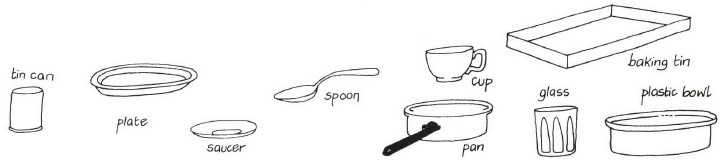
\includegraphics[width=12cm]{./img/vso/using-local-materials.jpg}
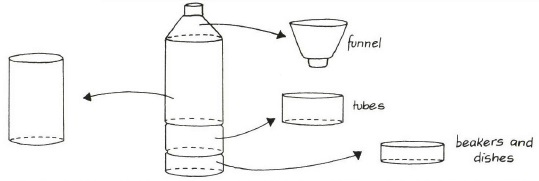
\includegraphics[width=12cm]{./img/vso/multi-purpose-bottle.jpg}
\end{center}


\begin{multicols}{2}

%\section{Alligator Clips}
%\label{sec:alligator-clips}
%\vspace{-10pt}
%\textbf{Use:} Connecting electrical components\\
%\textbf{Materials:} Clothespins, aluminum foil, glue\\
%\textbf{Procedure:} Glue aluminum foil around the clamping tips of a clothespin.

\section{Balance} \index{Beam balance}
\label{sec:balance}
\vspace{-10pt}
\textbf{Use:} Measuring mass\\
\textbf{Materials:} Ruler or wooden bar 30 cm $\times$ 2 cm, nails, razor/knife, string/wire, pen, 2 \nameref{sec:scale-pan}\\
\textbf{Procedure:} Find the balancing point of the ruler/wood block and mark it with a pen. Use a heated nail to make a hole through this point. Make notches at 5 cm intervals on either side of the center hole using a razor/knife to suspend scale pans. Use a string/wire tied through the center hole to suspend the balance.
\begin{center}
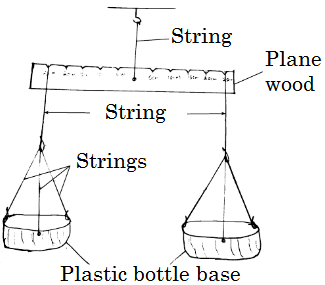
\includegraphics[width=0.4\textwidth]{./img/beam-balance-2.png}
\end{center}

\section{Beakers} \index{Beakers}
\label{sec:beakers}
\vspace{-10pt}
\textbf{Use:} To hold liquids, to heat liquids\\
\textbf{Materials:} Water bottles, jam jars, metal cans, knife\slash razor\\
\textbf{Procedure:} Take empty plastic bottles of different sizes. Cut them in half. The base can be used as a beaker. Jam jars made of glass, cut off metal cans and aluminum pots may be used when heating.\\
\textbf{Safety:} Glass containers may shatter if heated too much. Use standard laboratory equipment if extreme heating is needed.
\begin{center}
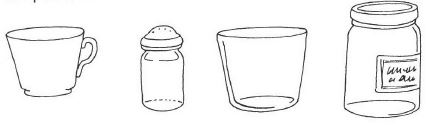
\includegraphics[width=8cm]{./img/vso/beakers.jpg}
\end{center} 

\section{Blowpipe} \index{Blowpipe}
\label{sec:blowpipe}
\vspace{-10pt}
\textbf{Use:} Increasing temperature of flames\\
\textbf{Materials:} Syringe needle, tube/straw/pen tube\\
\textbf{Procedure:} For sterilisation heat the needle
in open fire for a longer time before using it. A
drinking straw or a clean plastic tube can be
used as a connection to the mouth. 
\begin{center}
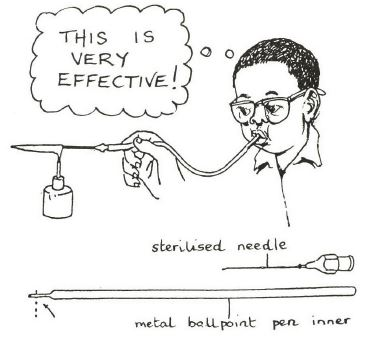
\includegraphics[width=0.4\textwidth]{./img/source/blowpipe.jpg}
\end{center} 

\columnbreak

%\section{Bulbs}
%\label{sec:lightbulbs}
%\vspace{-10pt}
%\textbf{Use:} Electrical circuits, diodes\\
%\textbf{Materials:} Broken phone chargers, flashlights, other electronic devices\\
%\textbf{Procedure:} Look for LEDs from broken items at hardware stores, local technicians, or small shops. 

\section{Bunsen Burner} \index{Bunsen burner|see{Heat sources}}
\label{sec:bunsen-burner}
See \nameref{sec:heatsources} (p.~\pageref{sec:heatsources}).

\section{Burettes} \index{Burettes}
\label{sec:burettes}
\vspace{-10pt}
\textbf{Use:} Titration

\subsection{Version 1}
\vspace{-6pt}
\textbf{Materials:} 10~mL syringes \\
\textbf{Procedure:} Use 10~mL disposable plastic syringes with 0.2~mL gradations. Students can estimate between the lines to at least 0.05~mL. If you must buy, buy plastic. 
%Note that broken burettes can often be repaired -- see \nameref{cha:burettes} (p.~\pageref{cha:burettes}).

\subsection{Version 2}
\vspace{-6pt}
\textbf{Materials:} Syringe, IV giving set, super glue, knife\\
\textbf{Procedure:} Cut off the part of the IV tube with the 
flow
control slider. Remove the plunger from the syringe and use superglue to
attach the tube to the nozzle of the syringe.
\begin{center}
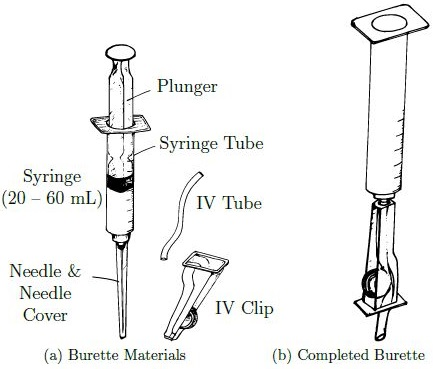
\includegraphics[width=0.49\textwidth]{./img/burette.jpg}
\end{center}

%\section{Circuit Components}
%\label{sec:circuit-comp}
%\vspace{-10pt}
%\textbf{Use:} Building simple circuits, Ohm's Law, amplifier, wave rectifiers\\
%\textbf{Materials:} Broken radio, computer, stereo, other electrical devices\\
%\textbf{Procedure:} Remove resistors, capacitors, transistors, diodes, motors, wires, transformers, inductors, rheostats, pulleys, gears, battery holders, switches, speakers and other components from the devices. Capacitors tend to state their capacitance in microFarads on their bodies.

%\section{Condenser}
%\label{sec:condenser}
%Pass clear plastic tubing through a water bottle filled 
%with cold water and prevent leaks with super glue. 
%If your condenser is under-performing (i.e. 
%steam comes out), 
%coil the plastic tubing so a greater length is in the water. 
%If your condenser is still under-performing 
%or you plan to use it for longer period of time, 
%devise a way to keep changing water inside the water bottle 
%to keep it from getting too hot. 
%Or, 
%submerge this condenser in a trough of water. 
%You could even run the plastic tubing through the sides of a bucket.

\section{Containers} \index{Containers}
\label{sec:containers}
\vspace{-10pt}
\textbf{Use:} Measuring large volumes (100~mL -- 2~L) of solution, titration, storage\\
\textbf{Materials:} Plastic water bottles, jars, tin cans\\
\textbf{Procedure:} Identify the volume of useful marks on the bottles 
and combine to measure accurate volumes.
\begin{center}
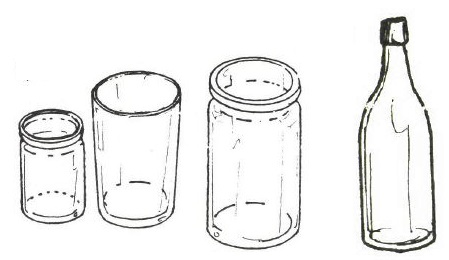
\includegraphics[width=0.4\textwidth]{./img/source/volumetric.jpg}
\end{center}

\section{Crucible} \index{Crucible}
\label{sec:crucible}
\vspace{-10pt}
\textbf{Use:} Heating substances at very high temperatures\\
\textbf{Materials:} 2 metal spoons, wire\\
\textbf{Procedure:} Place the material in one spoon and then wire 2 spoons together.
\begin{center}
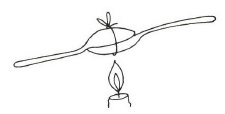
\includegraphics[width=0.4\textwidth]{./img/vso/crucible.jpg}
\end{center}

\section{Deflagrating Spoon} \index{Deflagrating spoon}
\label{sec:deflagratingspoon}
\vspace{-10pt}
\textbf{Use:} For heating chemicals to observe melting, decomposition, or other changes on heating\\
\textbf{Materials:} Metal spoons, galvanised wire, soda bottle cap\\
\textbf{Procedure:} Bend 30 cm of galvanised wire as shown. The wire should hold the bottle cap firmly.
\begin{center}
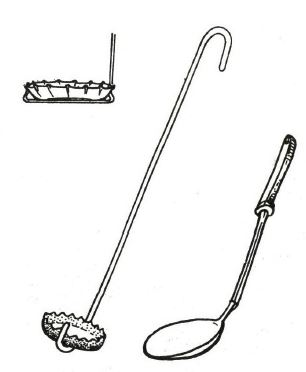
\includegraphics[width=0.3\textwidth]{./img/source/deflagrating-spoon.jpg}
\end{center}

\columnbreak

\section{Delivery Tube} \index{Delivery tube}
\label{sec:delivery-tube}
\vspace{-10pt}
\textbf{Use:} Movement and collection of gases, capillary tubes, hydraulic press\\
\textbf{Materials:} Straws, pen tubes, IV tubing (giving sets) from a pharmacy, bicycle tubing
\begin{center}
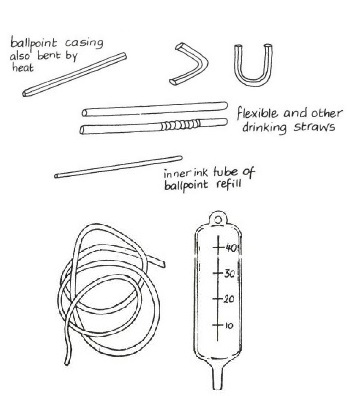
\includegraphics[width=0.45\textwidth]{./img/vso/tubes.jpg}
\end{center}

\section{Drawing Board} \index{Drawing board}
\label{sec:drawing-board}
\vspace{-10pt}
\textbf{Use:} Dissection, reflection, refraction of light\\
\textbf{Materials:} Thick cardboard

\section{Droppers} \index{Droppers}
\label{sec:droppers}
\vspace{-10pt}
\textbf{Use:} To transfer small amounts of liquid \\
\textbf{Materials:} 2 mL syringes, straws\\
\textbf{Procedure:} Take a syringe. Remove the needle to use as a dropper. Or insert a straw into a liquid and then plug the free end with a finger to remove a small amount and use as a dropper.

\section{Electrodes} \index{Electrodes}
\label{sec:electrodes}
\vspace{-10pt}
\textbf{Use:} Electrolysis
\begin{center}
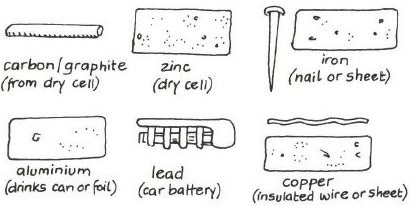
\includegraphics[width=0.45\textwidth]{./img/vso/electrodes.jpg}
\end{center}

\subsection{Graphite} \index{Graphite|see{Electrodes}}
\vspace{-6pt}
\textbf{Materials:} Old dry cell batteries\\
\textbf{Procedure:} Gently smash an old battery (D size) with a rock and pull out the electrode with pliers. DO NOT do this with alkaline batteries (most AA size) as they contain caustic liquids.

\columnbreak

\subsection{Zinc} \index{Zinc|see{Electrodes}}
\vspace{-6pt}
\textbf{Materials:} New dry cell batteries\\
\textbf{Procedure:} Carefully open up a NEW dry cell (D size) battery by peeling back the steel shell and slicing the plastic inside. You should find a cylindrical shell of zinc metal. Empty out the black powder inside (manganese dioxide mixed with zinc chloride and ammonium chloride; wash your hands after) and keep the graphite electrode for another day. The zinc shell should then be cut into strips, scraped clean, and boiled in water or washed with soap to remove any residual chemicals that might affect your experiment.
\begin{center}
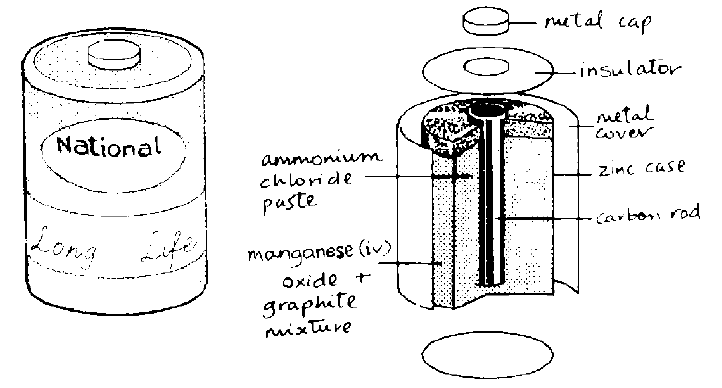
\includegraphics[width=0.4\textwidth]{./img/source/dry-cell.jpg}
\end{center}

\subsection{Iron} \index{Iron|see{Electrodes}}
\vspace{-6pt}
\textbf{Materials:} Ungalvanized nails from a hardware store
\subsection{Copper} \index{Copper|see{Electrodes}}
\vspace{-6pt}
\textbf{Materials:} Thick wire stripped of its insulation, also from a hardware store. Note that copper earthing rods have only a thin surface layer of copper these days.

%\section{Electrolytic cell}
%\label{sec:electrolytic-cell}
%Remove the plungers from two 10~mL syringes 
%and bore out the needle port with something sharp (knife, 
%thin pliers, 
%etc.). 
%Remove material gradually, 
%rotating the piece to ensure a circular cut. 
%When the hole is just big enough, 
%force through a graphite battery electrode 
%so 0.5-1~cm remains on the outside. 
%Twist the electrode during insertion to prevent it from snapping. 
%The gap should be air-tight, 
%but if the cut was too big or irregular 
%you can seal the holes with super glue. 
%Attach wires to the exposed part of the electrodes.
%
%To use the cell, 
%fill the tubes with your electrolyte solution 
%and place them wire end up in the cut off bottom of a large water bottle, 
%also filled with electrolyte solution. 
%Attach the wires to a power supply 
%(three or more 1.5~V dry cell batteries in series, 
%a 6~V motorcycle battery, 
%or a 12~V car battery) to start electrolysis. 
%The volume of gas produced at each electrode 
%may be measured by the gradations on the syringes, 
%and other products (copper metal plating, 
%iodine in solution) may be clearly observed.

%\section{Electrode Holders}
%\label{sec:electrode-holder}
%\vspace{-10pt}
%\textbf{Use:} Electrolysis\\
%\textbf{Materials:} Clothes pins
%\begin{center}
%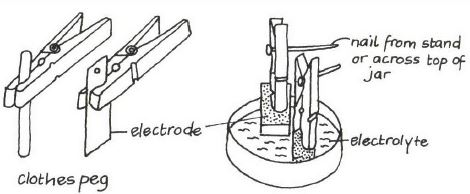
\includegraphics[width=0.49\textwidth]{./img/vso/electrode-holders.jpg}
%\end{center}

%\section{Eureka Can}
%\label{sec:eureka-can}
%\vspace{-10pt}
%\textbf{Use:} To measure volume of an irregular object, Archimedes' Principle, Law of Flotation\\
%\textbf{Materials:} Plastic bottle, knife, Optional: super glue, straw, nail, candle\\
%\textbf{Procedure:} Cut the top off of a 500 mL plastic bottle. Then cut a small strip at the top (1 cm wide by 3 cm long) and fold down to make a spout. Alternatively, heat a nail using a candle and poke a hole near the top of a cut off bottle. Super glue a straw so that it fits securely in the hole without leaking.
%\begin{center}
%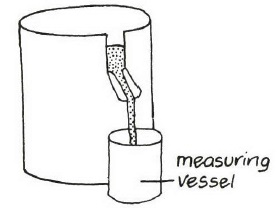
\includegraphics[width=5cm]{./img/vso/eureka-can.jpg}
%\end{center}

\columnbreak

\section{Filter Paper} \index{Filter paper}
\label{sec:filter-paper}
\vspace{-10pt}
\textbf{Use:} Filtration, separating mixtures, solutions\\
\textbf{Materials:} Cement bag paper, toilet paper, cloth
\begin{center}
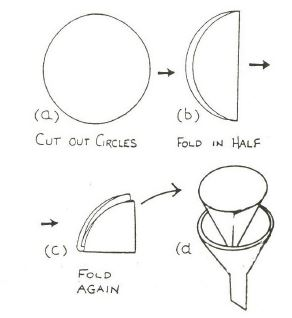
\includegraphics[width=0.4\textwidth]{./img/source/filter-paper.jpg}
\end{center}

\section{Flasks} \index{Flasks}
\label{sec:flasks}
\vspace{-10pt}
\textbf{Use:} Titrations, mixing solutions\\
\textbf{Materials:} Clean used liquor bottles, small water bottles\\
\textbf{Procedure:} When using these flasks for titrations, students must practice swirling enough that the solution remains well mixed. \\
\textbf{Safety:} When heating glass liquor bottles, make sure the cap is off.

\section{Funnel} \index{Funnel}
\label{sec:funnel}
\vspace{-10pt}
\textbf{Use:} To guide liquid or powder into a small opening\\
\textbf{Materials:} Empty water bottles, knife\\
\textbf{Procedure:} Take an empty water bottle and remove the cap. Cut it in half. The upper part of the bottle can be used as a funnel.  
\begin{center}
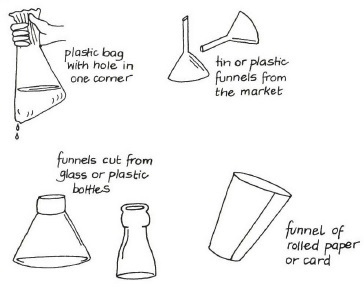
\includegraphics[width=0.49\textwidth]{./img/vso/funnels.jpg}
\end{center}

%\section{Glass blocks}
%\label{sec:glass-blocks}
%\vspace{-10pt}
%\textbf{Use:} Refraction of light\\
%\textbf{Materials:} 8~mm - 15~mm slabs of glass\\
%\textbf{Procedure:} Have a craftsman make rectangular pieces of glass with beveled edges, so students do not cut themselves. Glass blocks from a lab supply company are generally 15~mm thick. 8~mm and 10~mm glass is relatively common in towns. 12~mm and thicker glass exists though is even more difficult to find. Stack several pieces of thinner glass together and turn them on their edge.

\section{Gloves} \index{Gloves}
\label{sec:gloves}

\subsection{Latex gloves}
\vspace{-6pt}
\textbf{Use:} First aid, when one has open cuts on hands, handling specimens. They are worthless to the chemist because they make the hands less agile and give the user a false sense of security.\\
\textbf{Safety:} Concentrated acids and organic chemicals burn straight through latex.

\subsection{Thick gloves}
\vspace{-6pt}
\textbf{Use:} For working with organic solvents. Remember that the most dangerous organic solvents (benzene, carbon tetrachloride) should never be used in a school, with or without gloves. \\
\textbf{Materials:} Thick rubber gloves from village industry supply companies and some hardware stores\\
\textbf{Safety:} In general, avoid using chemicals that would make you want to wear gloves.

\section{Goggles} \index{Goggles}
\label{sec:goggles}
\vspace{-10pt}
\textbf{Use:} Handling concentrated acids\\
\textbf{Materials:} 1.5 L plastic water bottles, cardboard, sunglasses\\
\textbf{Procedure:} Cut a strip of plastic from a water bottle. Attach around your head with string or by using stiff cardboard as a frame. Goggles do not need to be impact resistant -- they just need to stand between hazardous chemicals and your eyes. 
\begin{center}
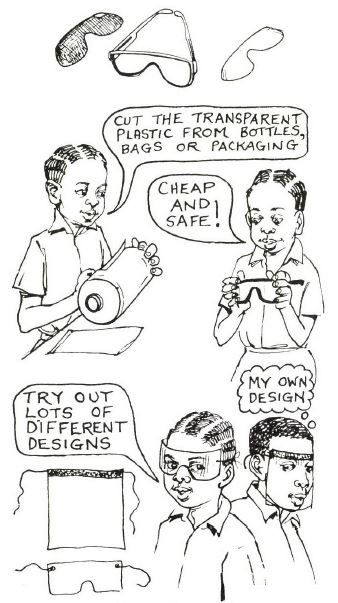
\includegraphics[width=0.4\textwidth]{./img/source/goggles.jpg}
\end{center}

\section{Heat Source} \index{Heat sources}
\label{sec:heatsources}
\vspace{-10pt}
\textbf{Use:} Heating substances\\
\textbf{Materials:} Candles, kerosene stoves, charcoal burners, Motopoa (alcohol infused heavy oil), butane lighters, spirit burners, metal can, bottle caps \\
Motopoa provides the best compromise heat source - it is the easiest to use and safest heat source with locally available burners.\\
\textbf{Procedure:} Cut a metal can in half or use a bottle cap and add a small amount of Motopoa.\\
\textbf{Safety:} Always have available fire-fighting equipment that you know how to use. Remember that to put out a Bunsen burner safely, you need to turn off the gas.
\begin{center}
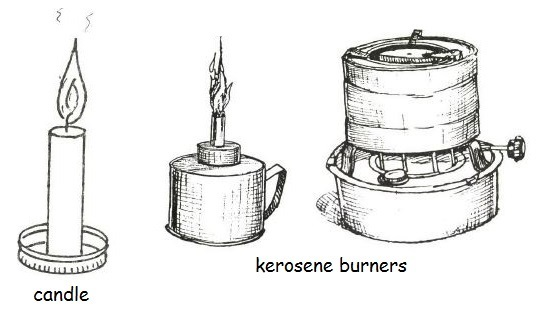
\includegraphics[width=0.49\textwidth]{./img/source/heat-sources.jpg}
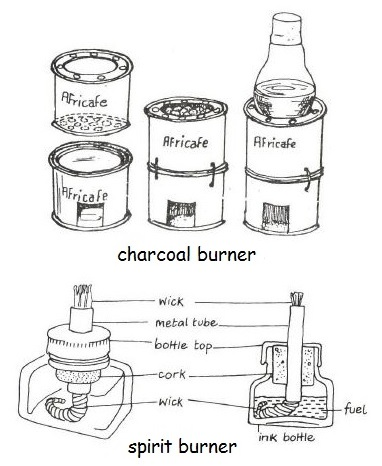
\includegraphics[width=0.49\textwidth]{./img/source/heat-sources-2.jpg}
\end{center}

\subsection{Heating Solutions}
The ideal heat source has a high heat rate (Joules transferred per second), 
little smoke, 
and cheap fuel, i.e. Motopoa.
A charcoal stove satisfies all of these 
but takes time to light and requires relatively frequent re-fueling. 
Kerosene stoves have excellent heat rates but are smoky. 

\subsection{Heating Solids}
The ideal heat source has a high temperature and no smoke, i.e. a Bunsen burner. 
For heating small objects for a short time (no more than 10-20 seconds), 
a butane lighter provides a very high temperature. 
Motopoa will provide a flame of satisfactory temperature 
for as long as necessary.

\subsection{Flame Tests}
The ideal heat source has a high temperature 
and produces a non-luminous flame, i.e. a Bunsen burner. 
Motopoa is next best – hot and non-luminous. 
Spirit burners produce a non-luminous flame at much greater cost, 
unless methylated spirits are used as fuel 
in which case the flame is much cooler. 
A butane lighter produces a very hot flame of sufficient size 
and time for flame tests although the non-luminous region is small. 
Kerosene stoves will work for some salts.

\section{Indicator} \index{Indicator}
\label{sec:indicator}
\vspace{-10pt}
\textbf{Use:} Determine presence of acid or base, determine pH\\
\textbf{Materials:} Rosella leaves, hot water, bottle\\
\textbf{Procedure:} Place some coloured leaves into a bottle of warm water to extract the colour. Use a straw to drop onto solutions or prepare indicator paper by dipping thing strips into the coloured solution. Rosella turns red for acids and greenish blue for bases.
\begin{center}
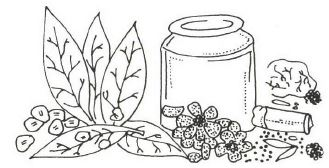
\includegraphics[width=0.4\textwidth]{./img/vso/making-indicators.jpg}
\end{center}

\section{Iron Filings} \index{Iron filings}
\label{sec:iron-filings}
\vspace{-10pt}
\textbf{Use:} To map magnetic fields\\
\textbf{Materials:} Steel wool / Iron wool used for cleaning pots\\
\textbf{Procedure:} Rub some steel wool between your thumb and fingers.  The small pieces that fall are iron filings.  Collect them in a matchbox or other container to use again.

\section{Masses} \index{Masses|see{Weights}}
\label{sec:masses}
See \nameref{sec:weights} (p.~\pageref{sec:weights}).

\section{Measuring Cylinder} \index{Measuring cylinder}
\label{sec:meascyl}
\vspace{-10pt}
\textbf{Use:} Measuring volume\\
\textbf{Materials:} Plastic bottles of different sizes, syringes (10 mL - 50 mL), fluorescent light tubes, marker pen, ruler, bucket of water\\
\textbf{Procedure:} Using the syringe, transfer a known volume of water from the bucket to the empty bottle. Use the marker pen to mark the level of water on the bottle. Repeat for a range of volumes, using a ruler to complete the scale. 
\begin{center}
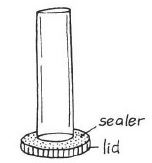
\includegraphics[width=0.2\textwidth]{./img/vso/meas-cyl.jpg}
\end{center}

\section{Metre Rule} \index{Metre rule}
\label{sec:meter-rule}
\vspace{-10pt}
\textbf{Use:} Measuring length\\
\textbf{Materials:} Slabs of wood, ceiling board, permanent pen\\
\textbf{Procedure:} Buy one, take it and a permanent pen to a carpenter, and leave with twenty. Measure each new one to the original rule to prevent compounding errors.

\section{Microscope}
\label{sec:microscope}
See \nameref{cha:microscopy} (p.~\pageref{cha:microscopy}).

%\section{Mirrors}
%\label{sec:mirrors}
%
%\subsection{Plane Mirrors}
%\vspace{-6pt}
%\textbf{Use:} Microscope, Laws of Reflection\\
%\textbf{Materials:} piece of thin glass, kibatari, super glue, small wooden blocks 
%
%\emph{Optional}: Small pieces of mirror glass are cheap or free at a glass cutter's shop\\
%\textbf{Procedure:} Light the kibatari so that it creates a lot of smoke.  Pass one side of the glass repeatedly over the kibatari until that side is totally black.  The other side acts as a mirror. Super glue to small wooden blocks to stand upright.
%
%\subsection{Curved Mirrors}
%\vspace{-6pt}
%\textbf{Use:} Curved mirror practicals\\
%\textbf{Materials:} Spoons\\
%\textbf{Procedure:} Inside surface is a concave mirror; back surface is a convex mirror.
%\begin{center}
%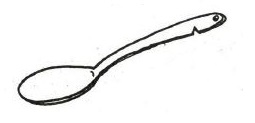
\includegraphics[width=0.2\textwidth]{./img/source/spoon.jpg}
%\end{center}

\section{Mortar and Pestle} \index{Mortar and pestle}
\label{sec:mortar-and-pestle}
\vspace{-10pt}
\textbf{Use:} To powder chemicals\\
\textbf{Materials:} 2 metal spoons, glass bottle\\
\textbf{Procedure:} Place chemicals between two nested metal spoons and grind down. 
Alternatively, crush chemicals on a sheet of paper by pressing on them with the bottom of a glass bottle.
\begin{center}
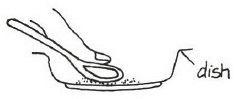
\includegraphics[width=5cm]{./img/vso/mortar-pestle.jpg}
\end{center}

%\section{Nichrome Wire}
%\label{sec:nichrome-wire}
%For flame tests in chemistry, 
%you can use a steel wire thoroughly scraped clean with iron or steel wool. 
%For physics experiments, 
%see \nameref{sec:wire} (p.~\pageref{sec:wire}).

\section{Optical Pins} \index{Optical pins}
\label{sec:optical-pins}
\vspace{-10pt}
\textbf{Use:} Compass needles, making holes, dissection, mirror practicals\\
\textbf{Materials:} Office pins, sewing needles, needles from syringes

\section{Pipettes} \index{Pipettes}
\label{sec:pipettes}
\vspace{-10pt}
\textbf{Use:} Transferring small amounts of liquid\\
\textbf{Materials:} Disposable plastic syringes (1, 2, 5, 10, 20, 25, 30 and 50 mL sizes)\\
\textbf{Procedure:} Suck first 1~mL of air and then put the syringe into the solution to suck up the liquid. There should be a flat meniscus under the layer of air.\\
\textbf{Safety:} Avoid standard pipettes to eliminate danger of mouth pipetting.
\begin{center}
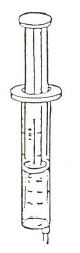
\includegraphics[width=0.1\textwidth]{./img/source/syringe.jpg}
\end{center}

%\section{Pulleys}
%\label{sec:pulleys}
%\vspace{-10pt}
%\textbf{Use:} Simple machines\\
%\textbf{Materials:} Bent nail, twisted wire, thread reel, water bottle, string, coat hanger\\
%\textbf{Procedure:} Cut off the top of a water bottle just below the lip where the top screws on. Run string or stiff wire through the centre to hang from a table or chair.
%\begin{center}
%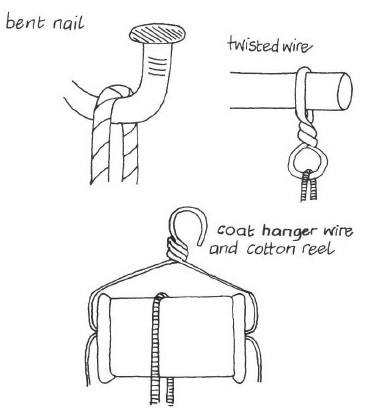
\includegraphics[width=0.4\textwidth]{./img/vso/pulleys.jpg}
%\end{center}

%\section{Resistors}
%\label{sec:resistors}
%\vspace{-10pt}
%\textbf{Use:} Electrical components\\
%\textbf{Materials:} Old radios, circuit boards, soldering iron\\
%\textbf{Procedure:} Remove resistors from old radios and circuit boards by melting the solder with a soldering iron or a stiff wire heated by a charcoal stove. If you need to know the ohms, the resistors tell you. Each has four strips (five if there is a quality band) and should be read with the silver or gold strip for tolerance on the right. Each color corresponds to a number:\\[10pt]
%
%\begin{tabular}{lll}
%black = 0 & yellow = 4 & violet = 7\\
%brown = 1 & green = 5 & gray = 8\\
%red = 2 & blue = 6 & white = 9\\
%orange = 3 & & \\[10pt]
%\end{tabular} 
%
%\noindent and additionally for the third stripe: gold = -1 and silver = -2. \\
%
%\noindent The first two numbers should be taken as a two digit number, so green-violet would be 57, red-black 20, etc. The third number should be taken as the power of ten (a $ 10^{n} $ term), so red-orange-yellow would be $ 23 \times 10^{4} = 230000 $, red-brown-black would be $ 21 \times 10^{0} = 21 $ and blue-gray-silver would be $ 68 \times 10^{-2} = 0.68 $. The unit is always ohms. The fourth and possibly fifth bands may be ignored.

\section{Retort Stand} \index{Retort stand}
\label{sec:retort-stand}
\vspace{-10pt}
\textbf{Use:} To hold springs, burettes, pendulums or other objects\\
\textbf{Materials:} Filled 1.5 L water bottle, straight bamboo stick, tape, marker\\
\textbf{Procedure:} Tape the bamboo stick across the top of the water bottle so that it reaches out ~20 cm to one side. Attach a small clamp if required or hang the object directly from the bamboo stick.

Alternatively, place a 1~cm piece of reinforcing rod in a paint can full of wet cement and let it dry. Then attach a boss head and clamp.

\section{Scale Pans} \index{Scale pans}
\label{sec:scale-pan}
\vspace{-10pt}
\textbf{Use:} Beam balance\\
\textbf{Materials:} Plastic bottle, cardboard box, string\\
\textbf{Procedure:} Cut off the bottom of a plastic bottle or cardboard box. Poke 3 or more holes near the top and tie string through each hole. Join strings and tie at the top to hang from a single point.
\begin{center}
\includegraphics[width=8cm]{./img/source/scale-pans.png}
\end{center}

\section{Scalpels} \index{Scalpels}
\label{sec:scalpels}
\vspace{-10pt}
\textbf{Use:} Dissection\\
\textbf{Materials:} Razor blades, tongue depressors, super glue\\
\textbf{Procedure:} Add a handle by gluing a tongue depressor on either side of the razor blade. Hold together with a rubber band until dry.\\
\textbf{Safety:} Dull blades should be discarded. Because students need to apply more pressure when using them, there is a greater risk of slipping and thus of cuts. Sharp tools are much safer. 
\begin{center}
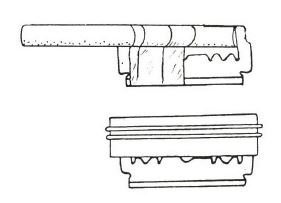
\includegraphics[width=0.4\textwidth]{./img/source/scalpel.jpg}
\end{center}

\section{Slides and Cover Slips} \index{Cover slips}
\label{sec:slide-cover-slip}
\vspace{-10pt}
\textbf{Use:} Microscopy\\
\textbf{Materials:} Small pieces of glass, stiff plastic\\
\textbf{Procedure:} Small piece of glass provides a slide for mounting the
specimen. Cover slips can be made
from thin (but stiff) transparent plastic from
display packing or bottles. Cut into small squares or circles.
\begin{center}
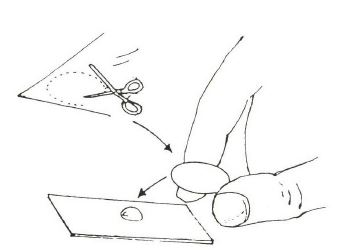
\includegraphics[width=0.4\textwidth]{./img/source/slide-cover-slip.jpg}
\end{center}

\section{Spatula} \index{Spatula}
\label{sec:spatula}
\vspace{-10pt}
\textbf{Use:} Transferring salts\\
\textbf{Materials:} Stainless steel spoons\\
\textbf{Procedure:} Use the handle end to remove salts from containers.\\
\textbf{Safety:} Clean all metal tools promptly after using with hydroxide, 
potassium manganate (VII), 
or manganese (IV) oxide. 
If the spoon corrodes, scrape with another spoon or steel wool.
\begin{center}
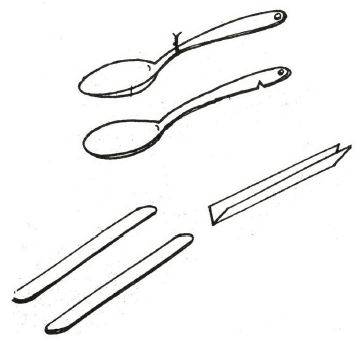
\includegraphics[width=0.4\textwidth]{./img/source/spatula.jpg}
\end{center}

%\section{Spring Balance}
%\label{sec:spring-balance}
%\textbf{Use:} To measure force applied on an object\\
%\textbf{Materials:} Strip of cardboard, rubber band, 2 paper clips, staple pin, pen\\
%\textbf{Procedure:} Cut a rubber band and fix one end to the top of a cardboard strip using a staple pin. (A stronger rubber band allows for a greater range of forces to measure.) Attach one paper clip near the top as a pointer. Attach the other paper clip as a hook at the bottom of the rubber band. Calibrate the spring balance using known masses. Write the equivalent force in Newtons on the cardboard. (A 1~g mass has a weight of 0.01 N, 100 g has a weight of 1 N, etc.)
%\begin{center}
%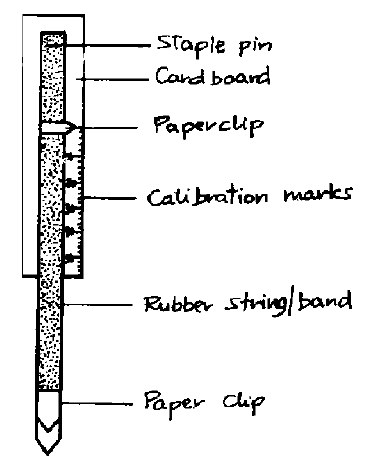
\includegraphics[width=0.4\textwidth]{./img/source/spring-balance.png}
%\end{center}

%\section{Springs}
%\label{sec:springs}
%\vspace{-10pt}
%\textbf{Use:} Hooke's Law, potential energy, work, spring balance\\
%\textbf{Materials:} Springs from hardware stores, bike stores, junk merchants in markets, window blinds; stiff wire; rubber bands; strips of elastic\\
%\textbf{Procedure:} Remove plastic covering if necessary and cut to a desired length (~5 cm). Alternatively wind a stiff wire around a marker pen or use rubber bands or elastic from a local tailor.

\section{Stoppers} \index{Stoppers}
\label{sec:stoppers}
\vspace{-10pt}
\textbf{Use:} To cover the mouth of a bottle, hold a capillary tube\\
\textbf{Materials:} Rubber from old tires or sandals, cork, plastic bottle cap, pen tube, super glue\\
\textbf{Procedure:} Cut a circular piece of rubber.  If the stopper is being used to hold a capillary tube, a hole can be melted in a plastic cap or rubber stopper. Alternatively, super glue a pen tube to a plastic bottle cap and connect to rubber tubing.
\begin{center}
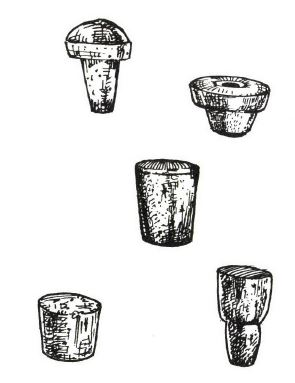
\includegraphics[width=0.3\textwidth]{./img/source/stoppers.jpg}
\end{center}

\section{Stopwatches} \index{Stopwatches}
\label{sec:stopwatches}
\vspace{-10pt}
\textbf{Use:} Simple pendulum, velocity, acceleration\\
\textbf{Materials:} Athletic and laboratory stopwatches from markets, digital wristwatches

\columnbreak

\section{Test Tubes} \index{Test tubes}
\label{sec:testtubes}

\subsection{Plastic Test Tubes}
\vspace{-6pt}
\textbf{Use:} To heat materials without a direct flame, to combine solutions\\
\textbf{Materials:} 10~mL syringes, matches\\
\textbf{Procedure:} Remove the needle and plunger from 10~mL syringes. Heat the end of the shell with a match until it melts. Press the molten end against a flat surface (like the end of the plunger) to fuse it closed. If the tube leaks, fuse it again. Test tubes made this way may be heated in a water bath up to boiling, hot enough for most experiments.
\begin{center}
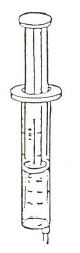
\includegraphics[width=0.1\textwidth]{./img/source/syringe.jpg}
\end{center}

\subsection{For Thermal Decomposition}
See \nameref{sec:deflagratingspoon} (p.~\pageref{sec:deflagratingspoon}).

\section{Test Tube Brush} \index{Test tubes! brushes}
\label{sec:test-tube-brush}
\vspace{-10pt}
\textbf{Use:} Cleaning test tubes\\
\textbf{Materials:} Sisal, wire\\
\textbf{Procedure:} Twist the wire around the sisal as shown or put a little sand in the test tube as an abrasive.
\begin{center}
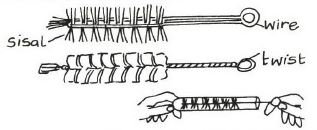
\includegraphics[width=0.45\textwidth]{./img/vso/test-tube-brush.jpg}
\end{center}

\section{Test Tube Holder / Tongs} \index{Test tubes! holders}
\label{sec:test-tube-holder}
\vspace{-10pt}
\textbf{Use:} To handle test tubes\\
\textbf{Materials:} Wooden clothespins, stiff wire, strip of paper or cloth\\
\textbf{Procedure:} Use clothespins or stiff wire for prolonged heating, or strips of paper or cloth for short-term heating.
\begin{center}
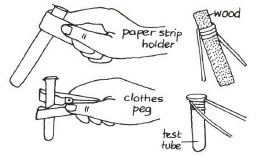
\includegraphics[width=0.45\textwidth]{./img/vso/test-tube-holder.jpg}
\end{center}

\section{Test Tube Racks} \index{Test tubes! racks}
\label{sec:test-tube-racks}
\vspace{-10pt}
\textbf{Use:} To hold test tubes vertically in place\\
\textbf{Materials:} Wire grid from local gardening store, styrofoam block, plastic bottle, sand, knife\\
\textbf{Procedure:} Fold a sheet of wire grid to make a table; punch holes in a piece of styrofoam; cut a plastic bottle in half and fill it with sand to increase stability. Or cut a plastic bottle along its vertical axis and rest the two cut edges on a flat surface. Cut holes into it for the test tubes.
\begin{center}
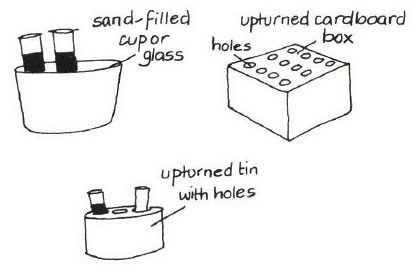
\includegraphics[width=0.45\textwidth]{./img/vso/test-tube-rack.jpg}
\end{center}

\section{Tripod Stands} \index{Tripod stands}
\label{sec:tripod-stands}
\vspace{-10pt}
\textbf{Use:} For supporting containers above heat sources, for elevating items\\
\textbf{Materials:} Stiff wire, metal rods, tin can\\
\textbf{Procedure:} Join bent pieces of thick wire together. Or cut the sides of a tin can to leave 3 legs.
\begin{center}
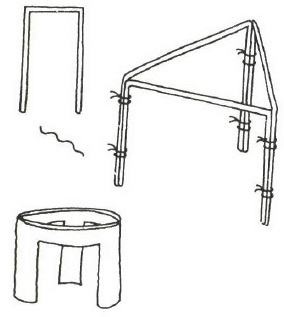
\includegraphics[width=5cm]{./img/vso/tripod-stand.jpg}
\end{center}

\section{Volumetric ``Glass''ware} \index{Volumetric glassware|see{Containers}}
\label{sec:volumetric-glassware}
See \nameref{sec:containers} (p.~\pageref{sec:containers}).

\section{Wash Bottle} \index{Wash bottle}
\label{sec:wash-bottle}
\vspace{-10pt}
\textbf{Use:} Washing hands after experiments\\
\textbf{Materials:} Water bottle, detergent, needle\\
\textbf{Procedure:} Put a hole in the cap of a water bottle using a syringe needle. 

\section{Water Bath} \index{Water bath}
\label{sec:hotwaterbathes}
\vspace{-10pt}
\textbf{Use:} To heat substances without using a direct flame\\
\textbf{Materials:} \nameref{sec:heatsources}, water, cooking pot\\
\textbf{Procedure:} Bring water to a boil in a small aluminum pot, then place the test tubes in the water to heat the substance inside the test tube. Prevent test tubes from falling over by clamping with clothespins or placing parallel wires across the container.
\begin{center}
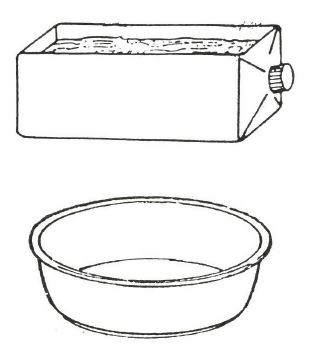
\includegraphics[width=0.4\textwidth]{./img/source/trough.jpg}
\end{center}

\section{Weights} \index{Weights}
\label{sec:weights}

\subsection{Crude Weights}
\vspace{-6pt}
\textbf{Use:} Concept of units, mass, weight\\
\textbf{Materials:} Batteries, coins, glass marbles from town, etc. \\
\textbf{Procedure:} Use objects of unknown mass to create new units and impart the concept of unit measure.

\subsection[Adding Weight in Known Intervals]{Adding Weight in Known \hfill \\ Intervals}
\vspace{-6pt}
\textbf{Use:} Hooke's Law practical\\
\textbf{Materials:} Water bottles, syringe\\
\textbf{Procedure:} Consider ``zero added mass'' the displacement of the pan with an empty water bottle. Then add masses of water in g equal to their volumes in mL (e.g. 50 mL = 50 g).

\subsection{Precise Weights}
\vspace{-6pt}
\textbf{Materials:} Plastic bags, sand, stones, 250 mL water bottles (all identical), tape, pen\\
\textbf{Procedure:} 
Use a beam balance and known masses at a market or nearby school to measure exact masses of bags of sand or stones.  Use a marker pen to mark the masses on the bags. 

If using water, use a beam balance from a nearby school to measure the exact mass of an empty water bottle. Add a volume of water in mL equal to the mass in g needed to reach a desired total mass. (The density of water is 1.0 g/mL.) This can be done precisely by using a plastic syringe. Label the bottle with tape and a pen.

\section{White Tiles} \index{White tiles}
\label{sec:white-tiles}
\vspace{-10pt}
\textbf{Use:} Titration\\
\textbf{Materials:} White paper\\
\textbf{Procedure:} If students are using syringes as burettes, they can also hold their flask up against a white wall.

%\section{Wire}
%\label{sec:wire}
%
%\subsection{Connecting Wires}
%\vspace{-6pt}
%\textbf{Use:} Connecting circuit components, current electricity\\
%\textbf{Materials:} Speaker wire, knife\\
%\textbf{Procedure:} Speaker wire can be found at any hardware store or taken from old appliances - the pairs of colored wires brained together. Strip using a knife, scissors or a wire stripper.
%\begin{center}
%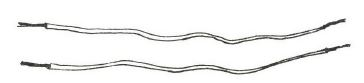
\includegraphics[width=0.4\textwidth]{./img/source/wire.jpg}
%\end{center}
%
%\subsection{Specific Gauge Wire}
%\vspace{-6pt}
%\textbf{Use:} Electrical components, motors, transformers, simple generators\\
%\textbf{Materials:} Copper wire without plastic covering (transformer wire), knife\slash scissors, matches\\
%\textbf{Procedure:} Scrape or burn off the insulating varnish at any points you wish to make electrical contact. 
%These wires come in a variety of diameters (gauges). A useful chart for converting diameter to gauge may be found at \url{http://www.dave-cushman.net/elect/wiregauge.html}. If the wire is sold by weight, 
%you can find the length if you know the diameter - the density of copper metal at room temperature is 8.94~g/cm$^{3}$. For example, with 0.375~mm wire, 250~g is about 63 metres.

\section{Wire Gauze} \index{Wire gauze}
\label{sec:wire-gauze}
\vspace{-10pt}
\textbf{Use:} Placing objects over heat\\
\textbf{Materials:} Tin can lid\\
\textbf{Procedure:} Poke holes in a tin can lid.
\begin{center}
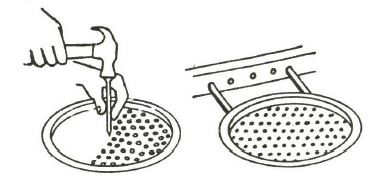
\includegraphics[width=0.4\textwidth]{./img/source/wire-gauze.jpg}
\end{center}

\end{multicols}














%\chapter{Local Materials List}
%\label{cha:local-materials}
%
%In order to gain a thorough understanding of science, students must be able to make a connection between classroom learning and the outside world. The application of scientific concepts to daily life is a critical component of a student's science education. The following is a list of locally available materials which may be used to substitute conventional materials and apparatus for various activities. These materials have the following advantages: 
%\begin{itemize*}
%\item They are readily available in the village or a nearby town;
%\item They are cheaper than conventional materials; 
%\item They may safely substitute the conventional materials without fear of losing accuracy or understanding; 
%\item They help students to draw a connection between science education and the world around them.
%\end{itemize*}
%Imagination and innovativeness is encouraged on the part of the student and teacher to find other suitable local substitutions. \\
%
%\noindent Throughout this book you will see materials that have been marked with an asterisk (*). These are locally available materials which can be made or purchased for your laboratory or classroom. The guide for using and making these local materials is found in this section.  
%
%\section{Balance}
%\label{sec:balance}
%\vspace{-10pt}
%\textbf{Use:} Measuring mass\\
%\textbf{Materials:} Ruler or wooden bar 30 cm $\times$ 2 cm, nails, \nameref{sec:heatsources}, razor/knife, string/wire, pen, 2 \nameref{sec:scalepans}\\
%\textbf{Procedure:} Find the balancing point of the ruler/wood block and mark it with a pen. Use a heated nail to make a hole through this point. Make notches at 5 cm intervals on either side of the center hole using a razor/knife to suspend scale pans. Use a string/wire tied through the center hole to suspend the balance.
%\begin{center}
%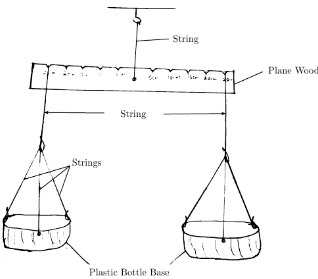
\includegraphics[width=8cm]{./img/beam-balance.png}
%\end{center}
%
%\section{Beakers}
%\label{sec:beakers}
%\vspace{-10pt}
%\textbf{Use:} To hold liquids, to heat liquids\\
%\textbf{Materials:} Water bottles, jam jars, metal cans, knife\slash razor\\
%\textbf{Procedure:} Take empty plastic bottles of different sizes. Cut them in half. The base can be used as a beaker. Jam jars made of glass, cut off metal cans and aluminum pots may be used when heating. 
%
%\section{Bunsen Burner}
%\label{sec:bunsen-burner}
%See \nameref{sec:heatsources}.
%
%\section{Burettes}
%\label{sec:burettes}
%\vspace{-10pt}
%\textbf{Use:} Titration\\
%\textbf{Materials:} 10~mL syringes \\
%\textbf{Procedure:} Use 10~mL disposable plastic syringes with 0.2~mL gradations. Students can estimate between the lines to at least 0.05~mL. If you must buy, buy plastic. Note that broken burettes can often be repaired -- see \nameref{cha:burettes}.
%
%\section{Crucible}
%\label{sec:crucible}
%\vspace{-10pt}
%\textbf{Use:} Heating substances at very high temperatures\\
%\textbf{Materials:} 2 metal spoons, wire\\
%\textbf{Procedure:} Place the material in one spoon and then wire 2 spoons together.
%\begin{center}
%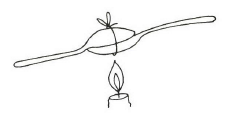
\includegraphics[width=6cm]{./img/crucible.png}
%\end{center}
%
%\section{Deflagrating Spoon}
%\label{sec:deflagratingspoon}
%\vspace{-10pt}
%\textbf{Use:} For heating chemicals to observe melting, decomposition, or other changes on heating\\
%\textbf{Materials:} Metal spoons\\
%
%\section{Delivery Tube}
%\label{sec:delivery-tube}
%\vspace{-10pt}
%\textbf{Use:} Movement and collection of gases, capillary tubes, hydraulic press\\
%\textbf{Materials:} Straws, pen tubes, IV tubing (giving sets) from a pharmacy, bicycle tubing
%\begin{center}
%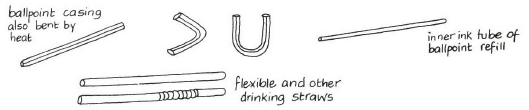
\includegraphics[width=12cm]{./img/tubes.png}
%\end{center}
%
%\section{Drawing Board}
%\label{sec:drawing-board}
%\vspace{-10pt}
%\textbf{Use:} Dissection\\
%\textbf{Materials:} Thick cardboard
%
%\section{Droppers}
%\label{sec:droppers}
%\vspace{-10pt}
%\textbf{Use:} To transfer small amounts of liquid \\
%\textbf{Materials:} 2 mL syringes, straws\\
%\textbf{Procedure:} Take a syringe. Remove the needle to use as a dropper. Or insert a straw into a liquid and then plug the free end with a finger to remove a small amount and use as a dropper.
%
%\section{Flasks}
%\label{sec:flasks}
%\vspace{-10pt}
%\textbf{Use:} Titrations, mixing solutions\\
%\textbf{Materials:} Clean used liquor bottles, small water bottles\\
%\textbf{Procedure:} When using these flasks for titrations, students must practice swirling enough that the solution remains well mixed. \\
%\textbf{Safety:} When heating glass liquor bottles, make sure the cap is off.
%
%\section{Funnel}
%\label{sec:funnel}
%\vspace{-10pt}
%\textbf{Use:} To guide liquid or powder into a small opening\\
%\textbf{Materials:} Empty water bottles, knife\\
%\textbf{Procedure:} Take an empty water bottle and remove the cap. Cut it in half. The upper part of the bottle can be used as a funnel.  
%\begin{center}
%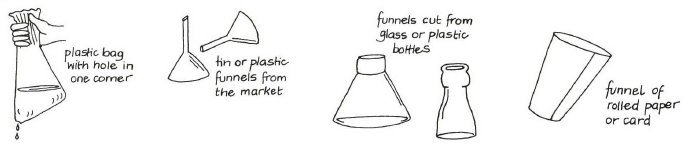
\includegraphics[width=12cm]{./img/funnels.png}
%\end{center}
%
%\section{Gloves}
%\label{sec:gloves}
%
%\subsection{Latex gloves}
%\vspace{-6pt}
%\textbf{Use:} First aid, when one has open cuts on hands, handling specimens. They are worthless to the chemist because they make the hands less agile and give the user a false sense of security.\\
%\textbf{Safety:} Concentrated acids and organic chemicals burn straight through latex.
%
%\subsection{Thick gloves}
%\vspace{-6pt}
%\textbf{Use:} For working with organic solvents. Remember that the most dangerous organic solvents (benzene, carbon tetrachloride) should never be used in a school, with or without gloves. \\
%\textbf{Materials:} Thick rubber gloves from village industry supply companies and some hardware stores\\
%\textbf{Safety:} In general, avoid using chemicals that would make you want to wear gloves.
%
%\section{Goggles}
%\label{sec:goggles}
%\vspace{-10pt}
%\textbf{Use:} Handling concentrated acids\\
%\textbf{Materials:} 1.5 L plastic water bottles, cardboard, sunglasses\\
%\textbf{Procedure:} Cut a strip of plastic from a water bottle. Attach around your head with string or by using stiff cardboard as a frame. Goggles do not need to be impact resistant -- they just need to stand between hazardous chemicals and your eyes. 
%
%\section{Heat Sources}
%\label{sec:heatsources}
%\vspace{-10pt}
%\textbf{Use:} Heating substances\\
%\textbf{Materials:} Candles, kerosene stoves, charcoal burners, Motopoa (alcohol infused heavy oil), butane lighters, spirit burners, metal can, bottle caps \\
%Motopoa provides the best compromise heat source - it is the easiest to use and safest heat source with locally available burners.\\
%\textbf{Procedure:} Cut a metal can in half or use a bottle cap and add a small amount of Motopoa.\\
%\textbf{Safety:} Always have available fire-fighting equipment that you know how to use. Remember that to put out a Bunsen burner safely, you need to turn off the gas.
%
%\subsection{Heating Solutions}
%The ideal heat source has a high heat rate (Joules transferred per second), 
%little smoke, 
%and cheap fuel, i.e. Motopoa.
%A charcoal stove satisfies all of these 
%but takes time to light and requires relatively frequent re-fueling. 
%Kerosene stoves have excellent heat rates but are smoky. 
%
%\subsection{Heating Solids}
%The ideal heat source has a high temperature and no smoke, i.e. a Bunsen burner. 
%For heating small objects for a short time (no more than 10-20 seconds), 
%a butane lighter provides a very high temperature. 
%Motopoa will provide a flame of satisfactory temperature 
%for as long as necessary.
%
%\subsection{Flame Tests}
%The ideal heat source has a high temperature 
%and produces a non-luminous flame, i.e. a Bunsen burner. 
%Motopoa is next best – hot and non-luminous. 
%Spirit burners produce a non-luminous flame at much greater cost, 
%unless methylated spirits are used as fuel 
%in which case the flame is much cooler. 
%A butane lighter produces a very hot flame of sufficient size 
%and time for flame tests although the non-luminous region is small. 
%Kerosene stoves will work for some salts.
%
%\section{Light Bulbs}
%\label{sec:lightbulbs}
%\vspace{-10pt}
%\textbf{Use:} Electrical circuits, diodes\\
%\textbf{Materials:} Broken phone chargers, flashlights, other electronic devices\\
%\textbf{Procedure:} Look for LEDs from broken items at hardware stores, local technicians, or small shops. 
%
%\section{Masses}
%\label{sec:masses}
%See \nameref{sec:weights}.
%
%\section{Measuring Cylinder}
%\label{sec:meascyl}
%\vspace{-10pt}
%\textbf{Use:} Measuring volume\\
%\textbf{Materials:} Plastic bottles of different sizes, syringes (10 mL - 50 mL), marker pen, ruler, bucket of water\\
%\textbf{Procedure:} Using the syringe, transfer a known volume of water from the bucket to the empty bottle. Use the marker pen to mark the level of water on the bottle. Repeat for a range of volumes, using a ruler to complete the scale. 
%
%\section{Mortar and Pestle}
%\label{sec:mortar-and-pestle}
%\vspace{-10pt}
%\textbf{Use:} To powder chemicals\\
%\textbf{Materials:} 2 metal spoons, glass bottle\\
%\textbf{Procedure:} Place chemicals between two nested metal spoons and grind down. 
%Alternatively, crush chemicals on a sheet of paper by pressing on them with the bottom of a glass bottle.
%\begin{center}
%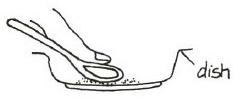
\includegraphics[width=5cm]{./img/mortar-pestle.png}
%\end{center}
%
%\section{Optical Pins}
%\label{sec:optical-pins}
%\vspace{-10pt}
%\textbf{Use:} Compass needles, making holes, dissection, mirror practicals\\
%\textbf{Materials:} Office pins, sewing needles, needles from syringes
%
%\section{Pipettes}
%\label{sec:pipettes}
%\vspace{-10pt}
%\textbf{Use:} Transferring small amounts of liquid\\
%\textbf{Materials:} Disposable plastic syringes (1, 2, 5, 10, 20, 25, 30 and 50 mL sizes)\\
%\textbf{Procedure:} Suck first 1~mL of air and then put the syringe into the solution to suck up the liquid. There should be a flat meniscus under the layer of air.\\
%\textbf{Safety:} Avoid standard pipettes to eliminate danger of mouth pipetting.
%
%\section{Retort Stand}
%\label{sec:retort-stand}
%\vspace{-10pt}
%\textbf{Use:} To hold springs, burettes, pendulums or other objects\\
%\textbf{Materials:} Filled 1.5 L water bottle, straight bamboo stick, tape, marker\\
%\textbf{Procedure:} Tape the bamboo stick across the top of the water bottle so that it reaches out ~20 cm to one side. Attach a small clamp if required or hang the object directly from the bamboo stick.
%
%Alternatively, place a 1~cm piece of reinforcing rod in a paint can full of wet cement and let it dry. Then attach a boss head and clamp.
%
%\section{Scale Pan}
%\label{sec:scale-pan}
%\vspace{-10pt}
%\textbf{Use:} Beam balance\\
%\textbf{Materials:} Plastic bottle, cardboard box, string\\
%\textbf{Procedure:} Cut off the bottom of a plastic bottle or cardboard box. Poke 3 or more holes near the top and tie string through each hole. Join strings and tie at the top to hang from a single point.
%\begin{center}
%\includegraphics[width=8cm]{./img/scale-pans.png}
%\end{center}
%
%\section{Scalpels}
%\label{sec:scalpels}
%\vspace{-10pt}
%\textbf{Use:} Dissection\\
%\textbf{Materials:} Razor blades, tongue depressors, super glue\\
%\textbf{Procedure:} Add a handle by gluing a tongue depressor on either side of the razor blade. Hold together with a rubber band until dry.\\
%\textbf{Safety:} Dull blades should be discarded. Because students need to apply more pressure when using them, there is a greater risk of slipping and thus of cuts. Sharp tools are much safer. 
%
%\section{Spatula}
%\label{sec:spatula}
%\vspace{-10pt}
%\textbf{Use:} Transferring salts\\
%\textbf{Materials:} Stainless steel spoons\\
%\textbf{Procedure:} Use the handle end to remove salts from containers.\\
%\textbf{Safety:} Clean all metal tools promptly after using with hydroxide, 
%potassium manganate (VII), 
%or manganese (IV) oxide. 
%If the spoon corrodes, scrape with another spoon or steel wool.
%
%\section{Stoppers}
%\label{sec:stoppers}
%\vspace{-10pt}
%\textbf{Use:} To cover the mouth of a bottle, hold a capillary tube\\
%\textbf{Materials:} Rubber from old tires or sandals, cork, plastic bottle cap, pen tube, super glue\\
%\textbf{Procedure:} Cut a circular piece of rubber.  If the stopper is being used to hold a capillary tube, a hole can be melted in a plastic cap or rubber stopper. Alternatively, super glue a pen tube to a plastic bottle cap and connect to rubber tubing.
%
%\section{Test Tubes}
%\label{sec:testtubes}
%
%\subsection{Plastic Test Tubes}
%\vspace{-6pt}
%\textbf{Use:} To heat materials without a direct flame, to combine solutions\\
%\textbf{Materials:} 10~mL syringes, matches\\
%\textbf{Procedure:} Remove the needle and plunger from 10~mL syringes. Heat the end of the shell with a match until it melts. Press the molten end against a flat surface (like the end of the plunger) to fuse it closed. If the tube leaks, fuse it again. Test tubes made this way may be heated in a water bath up to boiling, hot enough for most experiments.
%
%\subsection{For Thermal Decomposition}
%See \nameref{sec:deflagratingspoon}.
%
%\section{Test Tube Holder / Tongs}
%\label{sec:test-tube-holder}
%\vspace{-10pt}
%\textbf{Use:} To handle test tubes\\
%\textbf{Materials:} Wooden clothespins, stiff wire, strip of paper or cloth\\
%\textbf{Procedure:} Use clothespins or stiff wire for prolonged heating, or strips of paper or cloth for short-term heating.
%\begin{center}
%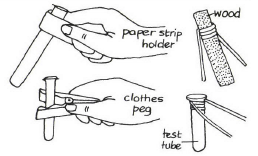
\includegraphics[width=8cm]{./img/test-tube-holder.png}
%\end{center}
%
%\section{Test Tube Racks}
%\label{sec:test-tube-racks}
%\vspace{-10pt}
%\textbf{Use:} To hold test tubes vertically in place\\
%\textbf{Materials:} Wire grid from local gardening store, styrofoam block, plastic bottle, sand, knife\\
%\textbf{Procedure:} Fold a sheet of wire grid to make a table; punch holes in a piece of styrofoam; cut a plastic bottle in half and fill it with sand to increase stability. Or cut a plastic bottle along its vertical axis and rest the two cut edges on a flat surface. Cut holes into it for the test tubes.
%\begin{center}
%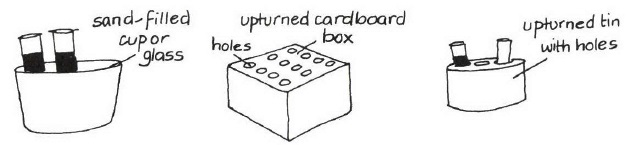
\includegraphics[width=12cm]{./img/test-tube-rack.png}
%\end{center}
%
%\section{Tripod Stands}
%\label{sec:tripod-stands}
%\vspace{-10pt}
%\textbf{Use:} For supporting containers above heat sources, for elevating items\\
%\textbf{Materials:} Stiff wire, metal rods, tin can\\
%\textbf{Procedure:} Join bent pieces of thick wire together. Or cut the sides of a tin can to leave 3 legs.
%\begin{center}
%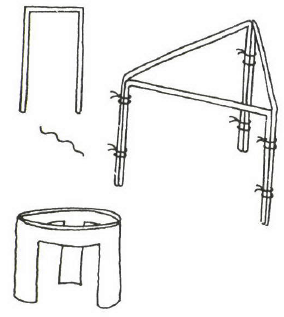
\includegraphics[width=5cm]{./img/tripod-stand.png}
%\end{center}
%
%\section{Volumetric ``Glass''ware}
%\label{sec:volumetric-glassware}
%\vspace{-10pt}
%\textbf{Use:} Measuring large volumes (100~mL -- 2~L) 
%of solution, titration\\
%\textbf{Materials:} Plastic water bottles \\
%\textbf{Procedure:} Identify the volume of useful marks on the bottles 
%and combine to measure accurate volumes.
%
%\section{Wash Bottle}
%\label{sec:wash-bottle}
%\vspace{-10pt}
%\textbf{Use:} Washing hands after experiments\\
%\textbf{Materials:} Water bottle, detergent, needle\\
%\textbf{Procedure:} Put a hole in the cap of a water bottle using a syringe needle. 
%
%\section{Water Bath}
%\label{sec:hotwaterbathes}
%\vspace{-10pt}
%\textbf{Use:} To heat substances without using a direct flame\\
%\textbf{Materials:} \nameref{sec:heatsources}, water, cooking pot\\
%\textbf{Procedure:} Bring water to a boil in a small aluminum pot, then place the test tubes in the water to heat the substance inside the test tube. Prevent test tubes from falling over by clamping with clothespins or placing parallel wires across the container.
%
%\section{Weights}
%\label{sec:weights}
%
%\subsection{Crude Weights}
%\vspace{-6pt}
%\textbf{Use:} Concept of units, mass, weight\\
%\textbf{Materials:} Batteries, coins, glass marbles from town, etc. \\
%\textbf{Procedure:} Use objects of unknown mass to create new units and impart the concept of unit measure.
%
%\subsection{Adding Weight in Known Intervals}
%\vspace{-6pt}
%\textbf{Use:} Hooke's Law practical\\
%\textbf{Materials:} Water bottles, syringe\\
%\textbf{Procedure:} Consider ``zero added mass'' the displacement of the pan with an empty water bottle. Then add masses of water in g equal to their volumes in mL (e.g. 50 mL = 50 g).
%
%\subsection{Precise Weights}
%\vspace{-6pt}
%\textbf{Materials:} Plastic bags, sand, stones, 250 mL water bottles (all identical), tape, pen\\
%\textbf{Procedure:} 
%Use a beam balance and known masses at a market or nearby school to measure exact masses of bags of sand or stones.  Use a marker pen to mark the masses on the bags. 
%
%If using water, use a beam balance from a nearby school to measure the exact mass of an empty water bottle. Add a volume of water in mL equal to the mass in g needed to reach a desired total mass. (The density of water is 1.0 g/mL.) This can be done precisely by using a plastic syringe. Label the bottle with tape and a pen.
%
%\section{White Tiles}
%\label{sec:white-tiles}
%\vspace{-10pt}
%\textbf{Use:} Titration\\
%\textbf{Materials:} White paper\\
%\textbf{Procedure:} If students are using syringes as burettes, they can also hold their flask up against a white wall.
%
%\section{Wire Gauze}
%\label{sec:wire-gauze}
%\vspace{-10pt}
%\textbf{Use:} Placing objects over heat\\
%\textbf{Materials:} Tin can lid\\
%\textbf{Procedure:} Poke holes in a tin can lid.
%\begin{center}
%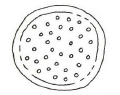
\includegraphics[width=4cm]{./img/wire-gauze.png}
%\end{center}